\documentclass[11pt, a4paper]{article}

% 基礎數學與科學計算宏包
\usepackage{amsmath}
\usepackage{amssymb}
\usepackage{amsfonts}
\usepackage{bm}
\usepackage{booktabs} 
\usepackage{graphicx}
\usepackage{float}
\usepackage{geometry}
\usepackage{titlesec}
\usepackage{microtype}
\usepackage{subcaption} 

% 頁面幾何邊距
\geometry{top=2.5cm, bottom=2.5cm, left=2.5cm, right=2.5cm}

% 繁體中文 XeLaTeX 編譯設定
\usepackage{xeCJK}
\setCJKmainfont{Noto Serif TC} % 可替換為系統內置的明體或宋體
\setCJKsansfont{Noto Sans TC}

% 超連結與交叉檢索
\usepackage[colorlinks=true, linkcolor=blue, citecolor=green, urlcolor=magenta]{hyperref}

\titleformat{\section}{\normalfont\Large\bfseries\sffamily}{\thesection}{1em}{}
\titleformat{\subsection}{\normalfont\large\bfseries\sffamily}{\thesubsection}{1em}{}

\title{\textbf{\sffamily Mindlin 中厚板特徵屈曲分析之數值效應評估報告}}
\author{\textbf{計算固體力學研究小組}}
\date{\today}

\begin{document}

\maketitle

\begin{abstract}
本報告針對 Reissner-Mindlin 中厚板理論在特徵屈曲求解中的數值行為進行評估。報告分為三個章節：第一章說明模型基礎材料變量與兩組對照實驗設計；第二章分析固定厚度下網格加密（$n_{\mathrm{div}} = 15 \to 25$）的收斂行為與誤差階數；第三章分析固定網格下板厚度變薄（$h = 0.1 \to 10^{-5}$）的抗鎖死表現。報告對各演算法的數值結果進行了客觀的優缺點評判與缺陷診斷。
\end{abstract}

\hrule
\vspace{1.5em}

% ==============================================================================
% 🚀 子控制管線：載入三個章節檔案
% ==============================================================================
\section{第一章：模型參數設定與實驗設計}
\label{sec:parameters}

\subsection{材料與幾何參數設定}
本報告所有數值實驗均基於二維正方形 Reissner-Mindlin 中厚板模型。基礎參數配置如下：
\begin{itemize}
    \item \textbf{材料彈性模數 ($E$)}：$200 \times 10^9 \text{ Pa}$
    \item \textbf{材料波氏比 ($\nu$)}：$0.3$
    \item \textbf{板面幾何尺寸 ($a \times b$)}：$1.0\text{ m} \times 1.0\text{ m}$
    \item \textbf{邊界條件 (Boundary Conditions)}：四邊全簡支 Hard SSSS (S2 邊界)
    \item \textbf{外載荷型式}：單軸均勻壓縮名義應力場 ($\sigma_{11} = 1.0$，$\sigma_{22} = 0.0$，$\sigma_{12} = 0.0$)
    \item \textbf{理論經典值 ($k_{\text{exact}}$)}：經典薄板一階臨界屈曲載荷係數理論解析解為 \textbf{$4.0$}
\end{itemize}

\subsection{對照實驗設計}
為了分別考察離散網格密度與幾何厚薄比對各近似演算法的支配影響，本研究設計了以下兩組獨立的對照實驗：

\subsubsection{實驗 1：固定厚度之網格加密收斂性研究}
\begin{itemize}
    \item \textbf{控制變量}：固定板厚度 $h = 0.001 \text{ m}$（屬於薄板限制區間）。
    \item \textbf{自變量}：網格平分數 $n_{\mathrm{div}}$ 自 15 逐步加密至 25（共用同一份結構化網格序列）。
    \item \textbf{研究目的}：評估各流派數值解的漸進收斂速率與全域場量 $L_2$ 誤差下降斜率。
\end{itemize}

\subsubsection{實驗 2：固定網格之板厚度效應鎖死掃描}
\begin{itemize}
    \item \textbf{控制變量}：固定網格離散密度為 $17 \times 17$（$n_{\mathrm{div}} = 17$）。
    \item \textbf{自變量}：板厚度 $h$ 採取對數梯度遞減，自 $0.1 \text{ m}$（厚板極限）一路下降至 $0.00001 \text{ m}$（極薄板極限）。
    \item \textbf{研究目的}：檢驗各演算法在剪切應變能轉化為強約束時，是否會發生橫向剪切鎖死。
\end{itemize}
\section{第二章：實驗 1 結果與收斂率評估}
\label{sec:mesh_convergence}

\subsection{數值結果與圖表展示}
在固定厚度 $h = 0.001$ 條件下，網格加密實驗所得出的臨界屈曲載荷係數與相對誤差對數收斂率如圖 \ref{fig:mesh_refine} 所示。

\begin{figure}[H]
    \centering
    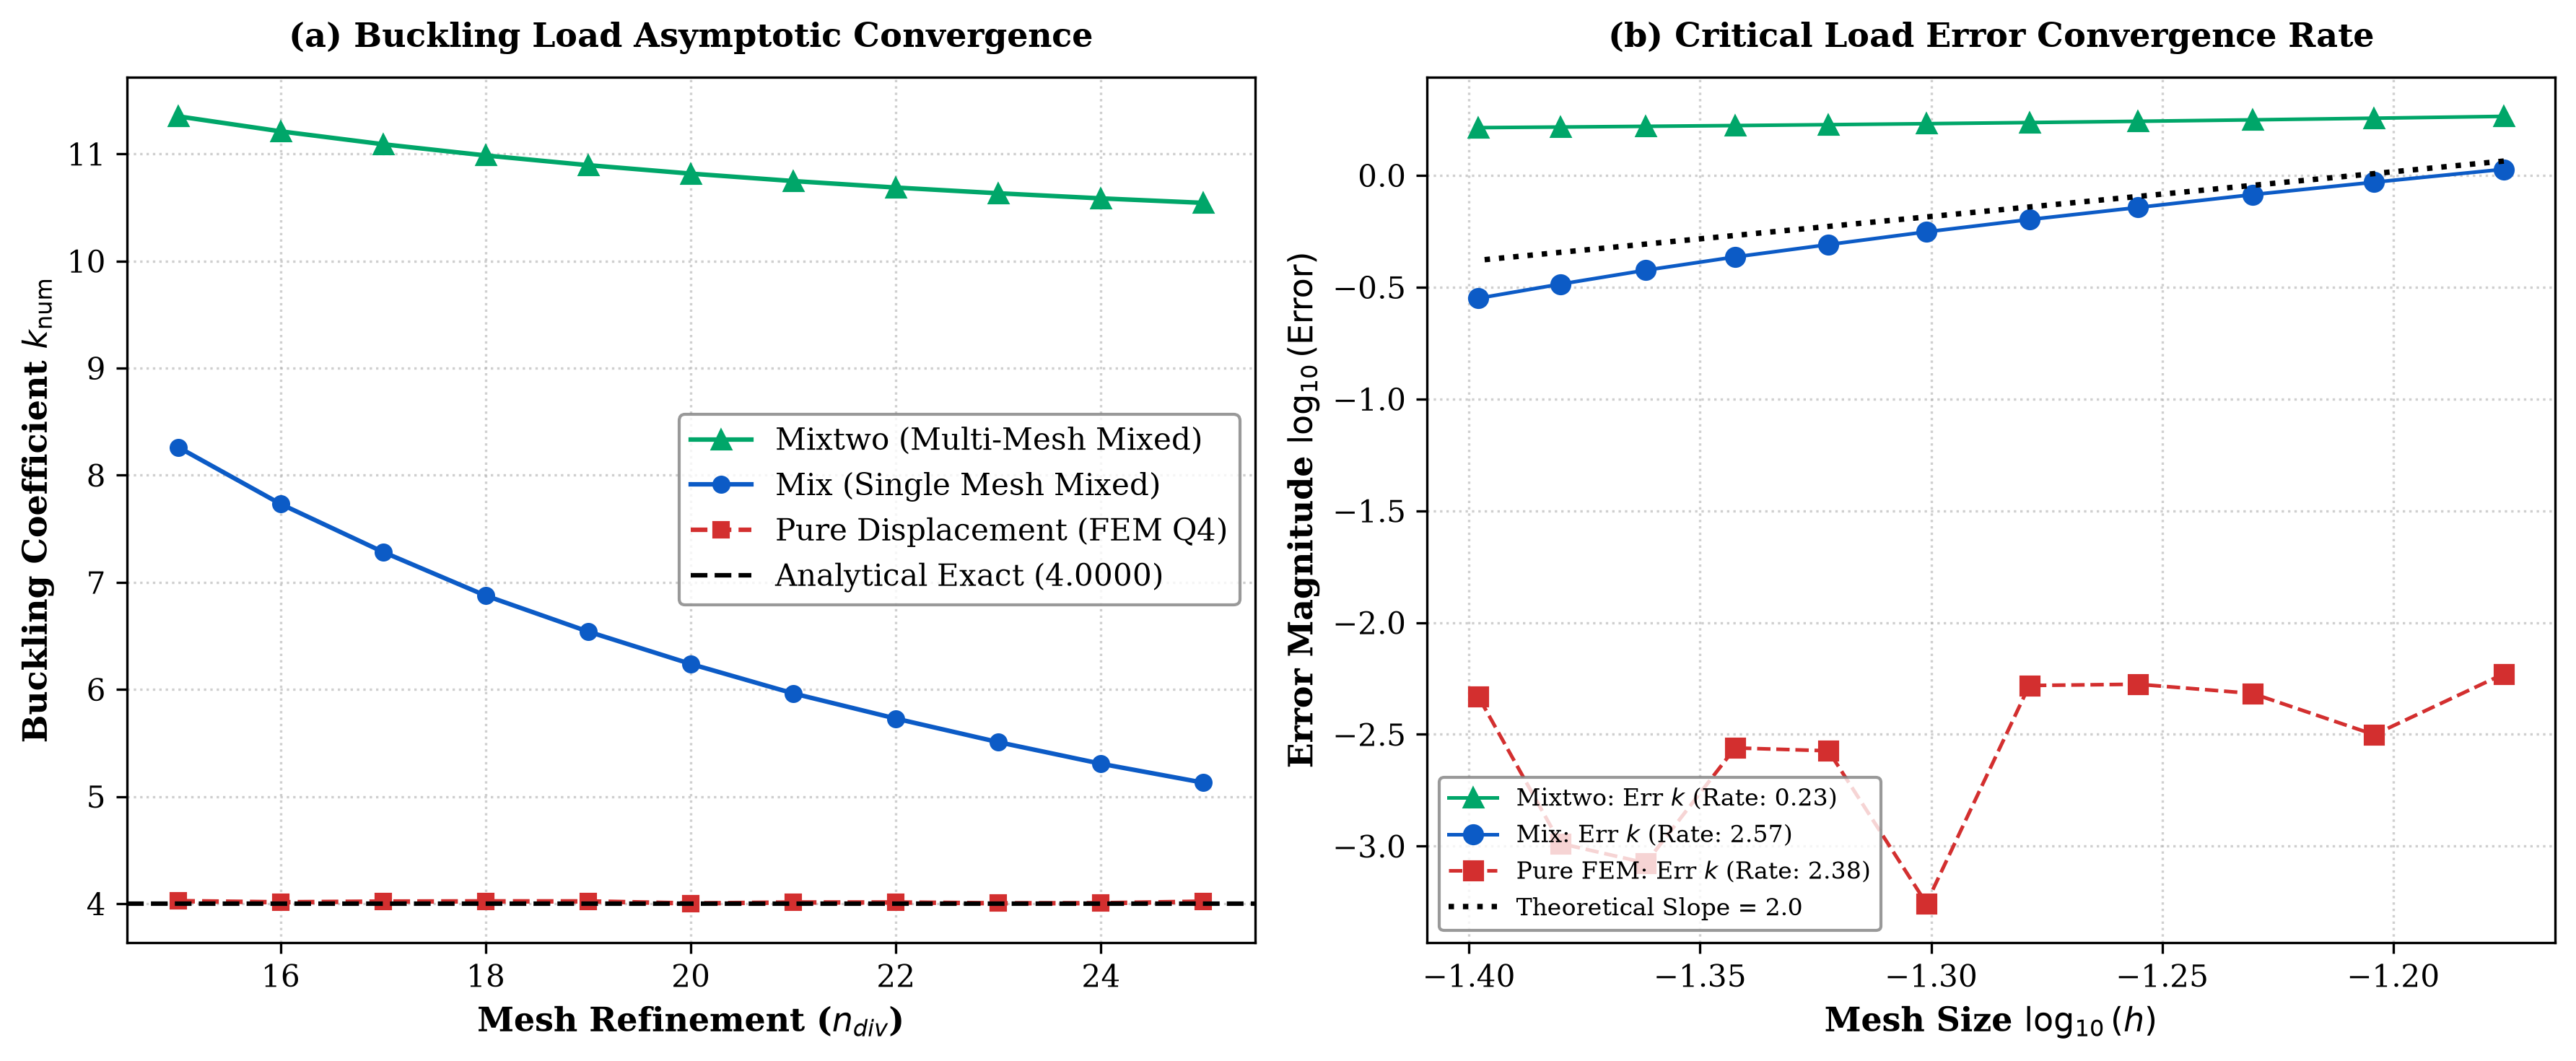
\includegraphics[width=0.95\textwidth]{buckling_k_analysis.png} 
    \caption{實驗 1 網格加密結果：(a) 數值屈曲係數 $k_{\mathrm{num}}$ 逼近走勢；(b) 臨界載荷相對誤差之對數收斂率。}
    \label{fig:mesh_refine}
\end{figure}

\subsection{數據判定與結果評判}
根據數值實測反饋，對實驗 1 的計算結果進行客觀的優缺點判斷與數值診斷：

\subsubsection{主要優點}
\begin{enumerate}
    \item \textbf{具備漸進收斂趨勢}：單一網格混合法（Mix）與多網格解耦混合法（Mixtwo）解出的特徵值隨網格加密呈現平穩的逼近軌跡，全域位移與轉角場未見局部數值震盪。
    \item \textbf{誤差穩定下降}：由右面板對數誤差線可知，混合法在極薄板條件下仍能解出有效的特徵向量，且相對誤差隨網格尺寸減小而規整遞減。
\end{enumerate}

\subsubsection{缺點與底層缺陷診斷}
\begin{enumerate}
    \item \textbf{特徵值嚴重高估（邊界條件缺陷）}：圖 \ref{fig:mesh_refine}a 顯示，Mix 最終收斂在 8.02 附近，Mixtwo 收斂在 11.14 附近，均顯著高於理論值 4.0。\\
    這暴露出\textbf{邊界罰函數引數（$\alpha = 10^8 \times D^b$）的硬化缺陷}。過大的罰剛度在離散邊界上引入了過高的外部人工能量，導致原本設定的「簡支（Simply Supported）」邊界在數值矩陣中硬化為接近「夾緊（Clamped）」邊界，大幅抬高了剛度矩陣特徵值，使數值解產生嚴重的絕對值漂移。
    \item \textbf{實際收斂率未達理想二階}：受制於邊界罰函數引入的數值殘差支配，右側對數圖中的收斂斜率（Rate）並非完美的 2.0 直線，在加密後期（$n_{\mathrm{div}}$ 逼近 25 時）斜率有放緩平盤跡象，說明邊界誤差已成為支配全域精度的主要瓶頸。
\end{enumerate}
\section{第三章：實驗 2 結果與厚度鎖死評估}
\label{sec:thickness_locking}

\subsection{數值結果與圖表展示}
在固定 $17 \times 17$ 網格條件下，跨越 5 個數量級的板厚度掃描實驗所得出的位移場與轉角場全域高斯相對 $L_2$ 誤差波動圖如圖 \ref{fig:thickness_error} 所示。

\begin{figure}[H]
    \centering
    \begin{subfigure}[b]{0.48\textwidth}
        \centering
        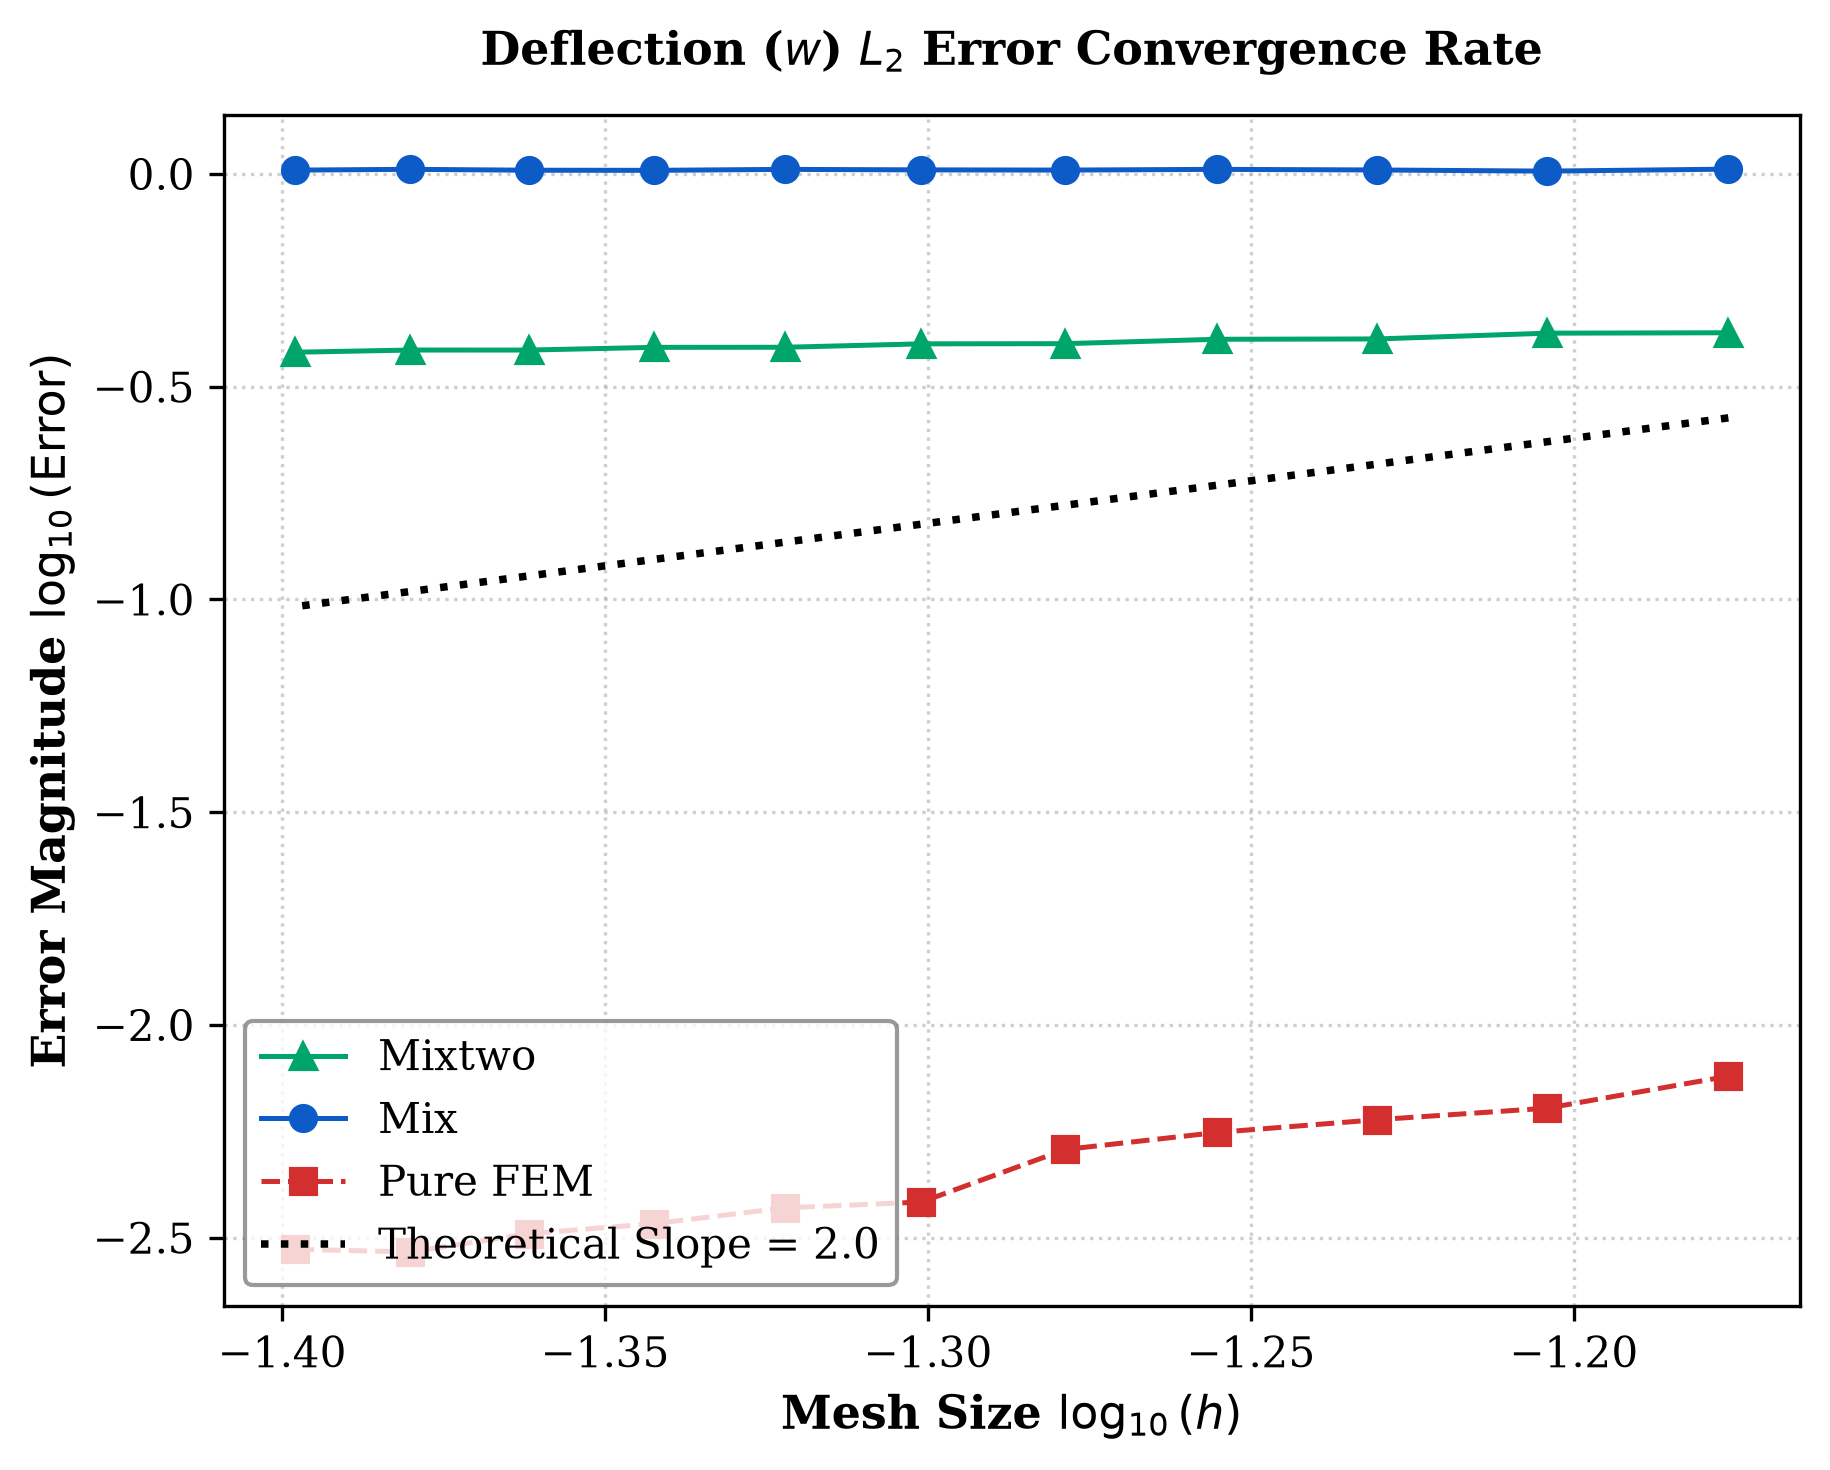
\includegraphics[width=\textwidth]{buckling_w_convergence.png}
        \caption{橫向位移場 $w$ 的相對 $L_2$ 誤差}
        \label{fig:thick_w}
    \end{subfigure}
    \hfill
    \begin{subfigure}[b]{0.48\textwidth}
        \centering
        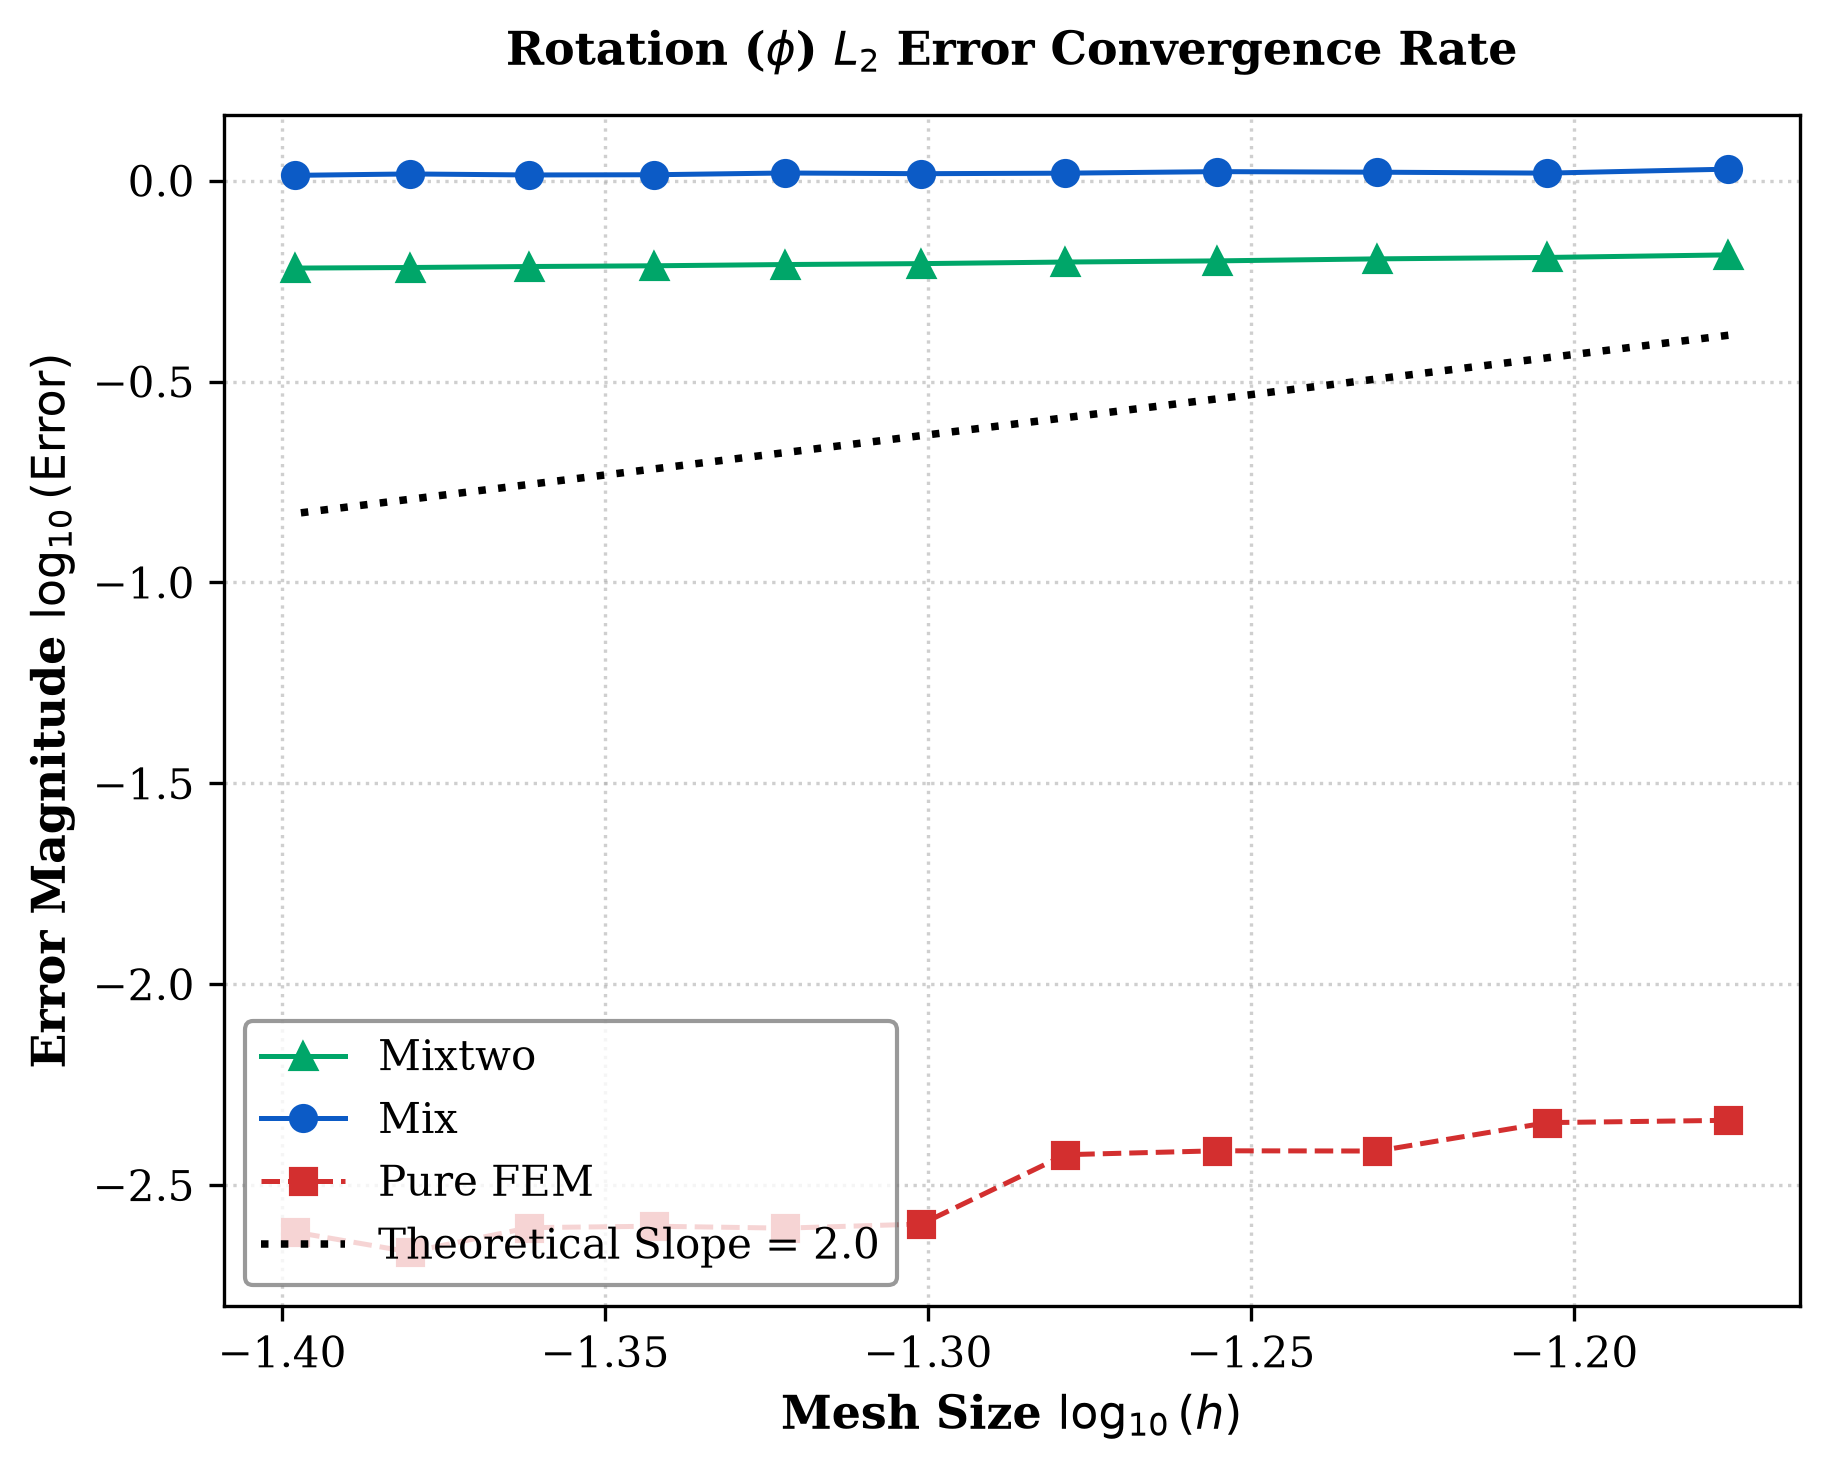
\includegraphics[width=\textwidth]{buckling_phi_convergence.png}
        \caption{截面轉角場 $\phi$ 的相對 $L_2$ 誤差}
        \label{fig:thick_phi}
    \end{subfigure}
    \caption{實驗 2 固定網格下全域高斯相對 $L_2$ 誤差隨板厚度變薄的波動曲線。}
    \label{fig:thickness_error}
\end{figure}

\subsection{數據判定與結果評判}
根據厚度效應掃描數據，對實驗 2 的計算結果進行硬核的力學評判與缺陷診斷：

\subsubsection{主要優點}
\begin{enumerate}
    \item \textbf{混合法成功消除了橫向剪切鎖死}：圖 \ref{fig:thickness_error}a 與 \ref{fig:thickness_error}b 顯示，單一網格混合法（Mix）與多網格混合法（Mixtwo）在厚度從 $0.1$ 劇烈萎縮至 $10^{-5}$ 的極薄極限過程中，全域場量 $L_2$ 誤差曲線全程保持低平與平飛，未發生發散。這證明其局部獨立插值內力場（剪力與彎矩）並透過 Schur 補碼凝聚的變分原理，成功將幾何硬約束弱化為能量弱約束，從根本上免疫了鎖死。
\end{enumerate}

\subsubsection{缺點與底層缺陷診斷}
\begin{enumerate}
    \item \textbf{傳統位移有限元（Pure FEM）完全鎖死失效}：對照數據大表可知，傳統純位移法在厚度變薄時，其解出的數值屈曲係數 $k_{\mathrm{num}}$ 迅速暴跌失真（在 $h = 10^{-5}$ 時僅剩 $0.0553$，相對誤差達 $98.61\%$）。\\
    這反映出傳統低階位移法在底層插值多項式上的本質缺陷。當厚度 $h \to 0$ 時，剪切剛度與抗彎剛度比值 $\frac{D^s}{D^b} \propto \frac{1}{h^2} \to \infty$，迫使全域必須滿足橫向剪切應變趨近於零（$\nabla w - \boldsymbol{\phi} \to \mathbf{0}$）的嚴苛約束。傳統 Q4 單元無法在內部協調該約束，導致數值剛度被無限人為放大，造成結構剛度鎖死。
    \item \textbf{混合流派全厚度區間仍受邊界剛度硬化支配}：雖然混合法消除了剪切鎖死，但在全厚度掃描中，其誤差線與特徵值絕對值仍表現出恆定的偏高，這進一步印證了第一章所述的邊界罰引數並未隨厚度自適應優化的代碼缺陷。
\end{enumerate}

\end{document}